% ============================================================
%  PRESENTACIÓN BEAMER – Dinámica Cuántica Computacional
%  Camilo Huertas  ·  Sebastián Rodriguez
%  Universidad Distrital Francisco José de Caldas
% ============================================================
\documentclass[aspectratio=169,10pt,xcolor=table]{beamer}

% ─── TEMA BASE ───────────────────────────────────────────────
\usetheme{Madrid}
\usecolortheme{default}

% ─── PALETA DE COLORES PERSONALIZADA ────────────────────────
\definecolor{UDprimary}{RGB}{0,60,120}      % azul institucional
\definecolor{UDsecond}{RGB}{220,50,50}      % rojo acento
\definecolor{UDlight}{RGB}{230,240,255}     % fondo claro
\definecolor{UDdark}{RGB}{20,30,60}         % texto oscuro
\definecolor{codegreen}{rgb}{0,0.55,0.2}
\definecolor{codegray}{rgb}{0.5,0.5,0.5}
\definecolor{codepurple}{rgb}{0.50,0,0.70}
\definecolor{backcolour}{RGB}{245,245,240}

% ─── APLICAR COLORES AL TEMA ─────────────────────────────────
\setbeamercolor{palette primary}{bg=UDprimary,fg=white}
\setbeamercolor{palette secondary}{bg=UDdark,fg=white}
\setbeamercolor{palette tertiary}{bg=UDsecond,fg=white}
\setbeamercolor{palette quaternary}{bg=UDprimary!80,fg=white}
\setbeamercolor{structure}{fg=UDprimary}
\setbeamercolor{section in toc}{fg=UDprimary}
\setbeamercolor{block title}{bg=UDprimary,fg=white}
\setbeamercolor{block body}{bg=UDlight}
\setbeamercolor{block title alerted}{bg=UDsecond,fg=white}
\setbeamercolor{block body alerted}{bg=UDsecond!10}
\setbeamercolor{block title example}{bg=UDprimary!70,fg=white}
\setbeamercolor{block body example}{bg=UDprimary!8}
\setbeamercolor{frametitle}{bg=UDprimary,fg=white}
\setbeamercolor{title}{fg=white}
\setbeamercolor{author}{fg=UDlight}
\setbeamercolor{date}{fg=UDlight}
\setbeamercolor{itemize item}{fg=UDsecond}
\setbeamercolor{itemize subitem}{fg=UDprimary}
\setbeamercolor{enumerate item}{fg=UDsecond}

% ─── FUENTES ─────────────────────────────────────────────────
\usepackage[T1]{fontenc}
\usepackage[utf8]{inputenc}
\usepackage[spanish]{babel}
\usepackage{lmodern}
\usepackage{microtype}

% ─── PAQUETES ESENCIALES ─────────────────────────────────────
\usepackage{amsmath,amssymb}
\usepackage{graphicx}
\usepackage{booktabs}
\usepackage{tabularx}
\usepackage{multirow}
\usepackage{listings}
\usepackage{tikz}
\usetikzlibrary{shapes.geometric,arrows.meta,positioning,shadows,fit}

% ─── ESTILO DE CÓDIGO ────────────────────────────────────────
\lstdefinestyle{fortranBeamer}{
  backgroundcolor=\color{backcolour},
  commentstyle=\color{codegreen}\itshape,
  keywordstyle=\color{UDprimary}\bfseries,
  keywordstyle=[2]\color{UDsecond}\bfseries,
  numberstyle=\tiny\color{codegray},
  stringstyle=\color{codepurple},
  basicstyle=\ttfamily\tiny, 
  breakatwhitespace=false,
  breaklines=true,
  captionpos=b,
  keepspaces=true,
  numbers=left,
  numbersep=4pt,
  showspaces=false,
  showstringspaces=false,
  tabsize=2,
  frame=single,
  rulecolor=\color{UDprimary!40},
  xleftmargin=8pt,
  xrightmargin=4pt,
  literate={á}{{\'a}}1 {é}{{\'e}}1 {í}{{\'i}}1 {ó}{{\'o}}1 {ú}{{\'u}}1
           {Á}{{\'A}}1 {É}{{\'E}}1 {Í}{{\'I}}1 {Ó}{{\'O}}1 {Ú}{{\'U}}1
           {ñ}{{\~n}}1 {Ñ}{{\~N}}1
}
\lstset{style=fortranBeamer}

% ─── PROGRESO Y NUMERACIÓN ───────────────────────────────────
\setbeamertemplate{navigation symbols}{}
\setbeamertemplate{footline}{%
  \leavevmode
  \hbox{%
    \begin{beamercolorbox}[wd=.30\paperwidth,ht=2.5ex,dp=1.125ex,leftskip=2pt]{palette secondary}%
      \usebeamerfont{author in head/foot}\insertshortauthor
    \end{beamercolorbox}%
    \begin{beamercolorbox}[wd=.45\paperwidth,ht=2.5ex,dp=1.125ex,center]{palette tertiary}%
      \usebeamerfont{title in head/foot}\insertshorttitle
    \end{beamercolorbox}%
    \begin{beamercolorbox}[wd=.25\paperwidth,ht=2.5ex,dp=1.125ex,rightskip=4pt plus1fil]{palette primary}%
      \usebeamerfont{date in head/foot}\hfill
      \insertframenumber{} / \inserttotalframenumber
    \end{beamercolorbox}%
  }%
}

\setbeamertemplate{headline}{%
  \begin{beamercolorbox}[ht=1.6ex,dp=0.4ex,wd=\paperwidth]{palette quaternary}%
    \hspace{6pt}{\tiny\color{white}\insertsectionhead}
    \hfill
    \begin{tikzpicture}[overlay]
      \fill[UDsecond] (0,0) rectangle (\paperwidth * \insertframenumber / \inserttotalframenumber, 0.8pt);
    \end{tikzpicture}
  \end{beamercolorbox}%
}

% ─── BULLETS PERSONALIZADOS ──────────────────────────────────
\setbeamertemplate{itemize item}{\color{UDsecond}\tiny\raisebox{1pt}{$\blacksquare$}}
\setbeamertemplate{itemize subitem}{\color{UDprimary}\tiny$\triangleright$}
\setbeamertemplate{enumerate item}{\color{UDsecond}\bfseries\insertenumlabel.}

% ─── METADATOS ───────────────────────────────────────────────
\title[Dinámica Cuántica Computacional]{%
  \textbf{Optimización y Paralelización}\\
  \large Dinámica Cuántica en 1D
}
\subtitle{Sistemas Distribuidos — Computación de Alto Desempeño}
\author[Huertas · Rodriguez]{%
  \textbf{Camilo Huertas} \quad \textbf{Sebastián Rodriguez}\\
  {\small Proyecto Curricular de Física}
}
\institute[UDFJC]{%
  Universidad Distrital Francisco José de Caldas\\
  {\small Docente: Carlos Andrés Gómez Vasco}
}
\date{27 de marzo de 2026}

% ============================================================
\begin{document}
% ============================================================

% ─── PORTADA ─────────────────────────────────────────────────
{
\setbeamertemplate{headline}{}
\setbeamertemplate{footline}{}
\begin{frame}[plain]
  \begin{tikzpicture}[remember picture,overlay]
    \fill[UDprimary] (current page.south west) rectangle (current page.north east);
    \fill[UDdark,opacity=0.5]
      (current page.south west) rectangle (current page.north east);
    \fill[UDsecond,opacity=0.85]
      ([xshift=-0.08\paperwidth]current page.north east) rectangle
      (current page.south east);
    \draw[UDlight,line width=1.5pt]
      ([yshift=-0.35\paperheight]current page.north west) --
      ([yshift=-0.35\paperheight,xshift=-0.08\paperwidth]current page.north east);
  \end{tikzpicture}

  \vspace{0.6cm}
  \begin{columns}[c]
    \column{0.18\textwidth}
       % \includegraphics[width=2.1cm]{../../img/logoUD2.png} % Descomenta si tienes el logo en img/
    \column{0.82\textwidth}
      {\color{white}\Large\bfseries Optimización y Paralelización}\\[4pt]
      {\color{UDsecond!80!white}\large\bfseries Dinámica Cuántica en 1D}\\[8pt]
      \color{white}\rule{0.9\textwidth}{0.4pt}\\[6pt]
      {\color{UDlight}\small Sistemas Distribuidos — Computación de Alto Desempeño}\\[10pt]
      {\color{white}\normalsize\textbf{Camilo Huertas} \quad \textbf{Sebastián Rodriguez}}\\
      {\color{UDlight}\small Proyecto Curricular de Física}\\[6pt]
      {\color{UDlight}\footnotesize Universidad Distrital Francisco José de Caldas}\\
      {\color{UDlight}\footnotesize Docente: Carlos Andrés Gómez Vasco \quad|\quad 27 de marzo de 2026}
  \end{columns}
\end{frame}
}

% ─── TABLA DE CONTENIDOS ─────────────────────────────────────
\begin{frame}{Contenido}
  \begin{columns}[t]
    \column{0.5\textwidth}
      \tableofcontents[sections={1-3}]
    \column{0.5\textwidth}
      \tableofcontents[sections={4-6}]
  \end{columns}
\end{frame}

% ============================================================
\section{El Problema Físico}
% ============================================================

\begin{frame}[shrink=5]{Descripción del Problema Físico}
  \begin{block}{Ecuación de Schrödinger Dependiente del Tiempo}
    Simulación de la evolución de un paquete de ondas gaussiano interactuando con un potencial escalar $V(x)$, empleando unidades atómicas ($\hbar=1$):
    \vspace{-0.2cm}
    \[
      i \frac{\partial \psi(x,t)}{\partial t} = \hat{H} \psi(x,t) \quad \text{donde} \quad \hat{H} = -\frac{1}{2m}\frac{\partial^2}{\partial x^2} + V(x)
    \]
  \end{block}

  \vspace{0.1cm}
  \begin{columns}[t]
    \column{0.48\textwidth}
      \begin{block}{El Reto Computacional}
        Aplicar el operador de evolución discreto:
        \[ \hat{U}(t) = e^{-i\hat{H}t} \]
        \textbf{Condición inquebrantable:} El método debe ser estrictamente unitario.
      \end{block}
    \column{0.48\textwidth}
      \begin{alertblock}{Restricción Física (Unitariedad)}
        La probabilidad total de encontrar la partícula debe conservarse en cada iteración temporal:
        \[ \int |\psi(x,t)|^2 dx = 1 \]
      \end{alertblock}
  \end{columns}
\end{frame}

% ============================================================
\section{Métodos Numéricos}
% ============================================================

\begin{frame}{Justificación de los Métodos Numéricos}
  \begin{columns}[t]
    \column{0.48\textwidth}
      \begin{block}{1. Pseudo-Espectral (FFT) - Base}
        Separa componentes cinética y potencial usando Fourier.
        \begin{itemize}
          \item \textbf{Pro:} Convergencia espectral espacial.
          \item \textbf{Contra:} Accesos a memoria no locales $\mathcal{O}(N \log N)$ imponen un techo de caché.
        \end{itemize}
      \end{block}
      
      \begin{block}{2. Aproximación de Cayley - Base}
        Esquema implícito análogo a Crank-Nicolson.
        \begin{itemize}
          \item \textbf{Pro:} Unitariedad incondicional.
          \item \textbf{Contra:} Sistemas tridiagonales crean dependencias de datos fatales para paralelizar.
        \end{itemize}
      \end{block}
      
    \column{0.48\textwidth}
      \begin{exampleblock}{3. Expansión de Chebyshev - Propuesta}
        Expansión polinomial del operador.
        \begin{itemize}
          \item \textbf{Pro:} Diferencias finitas. Excelente localidad espacial de datos (SIMD friendly).
          \item \textbf{Contra:} Limitado espectralmente.
        \end{itemize}
      \end{exampleblock}
      
      \begin{exampleblock}{4. Krylov-Lanczos - Propuesta}
        Proyección de $\hat{H}$ en subespacios ortonormales reducidos.
        \begin{itemize}
          \item \textbf{Pro:} Escala como $\mathcal{O}(m \cdot N)$. Máxima densidad de operaciones vectoriales y unitariedad estricta.
        \end{itemize}
      \end{exampleblock}
  \end{columns}
\end{frame}

% ============================================================
\section{Optimización Serial}
% ============================================================

\begin{frame}{Optimización Serial: Flags y la Ilusión del Tiling}
  \begin{columns}[c]
    \column{0.55\textwidth}
      \begin{figure}
        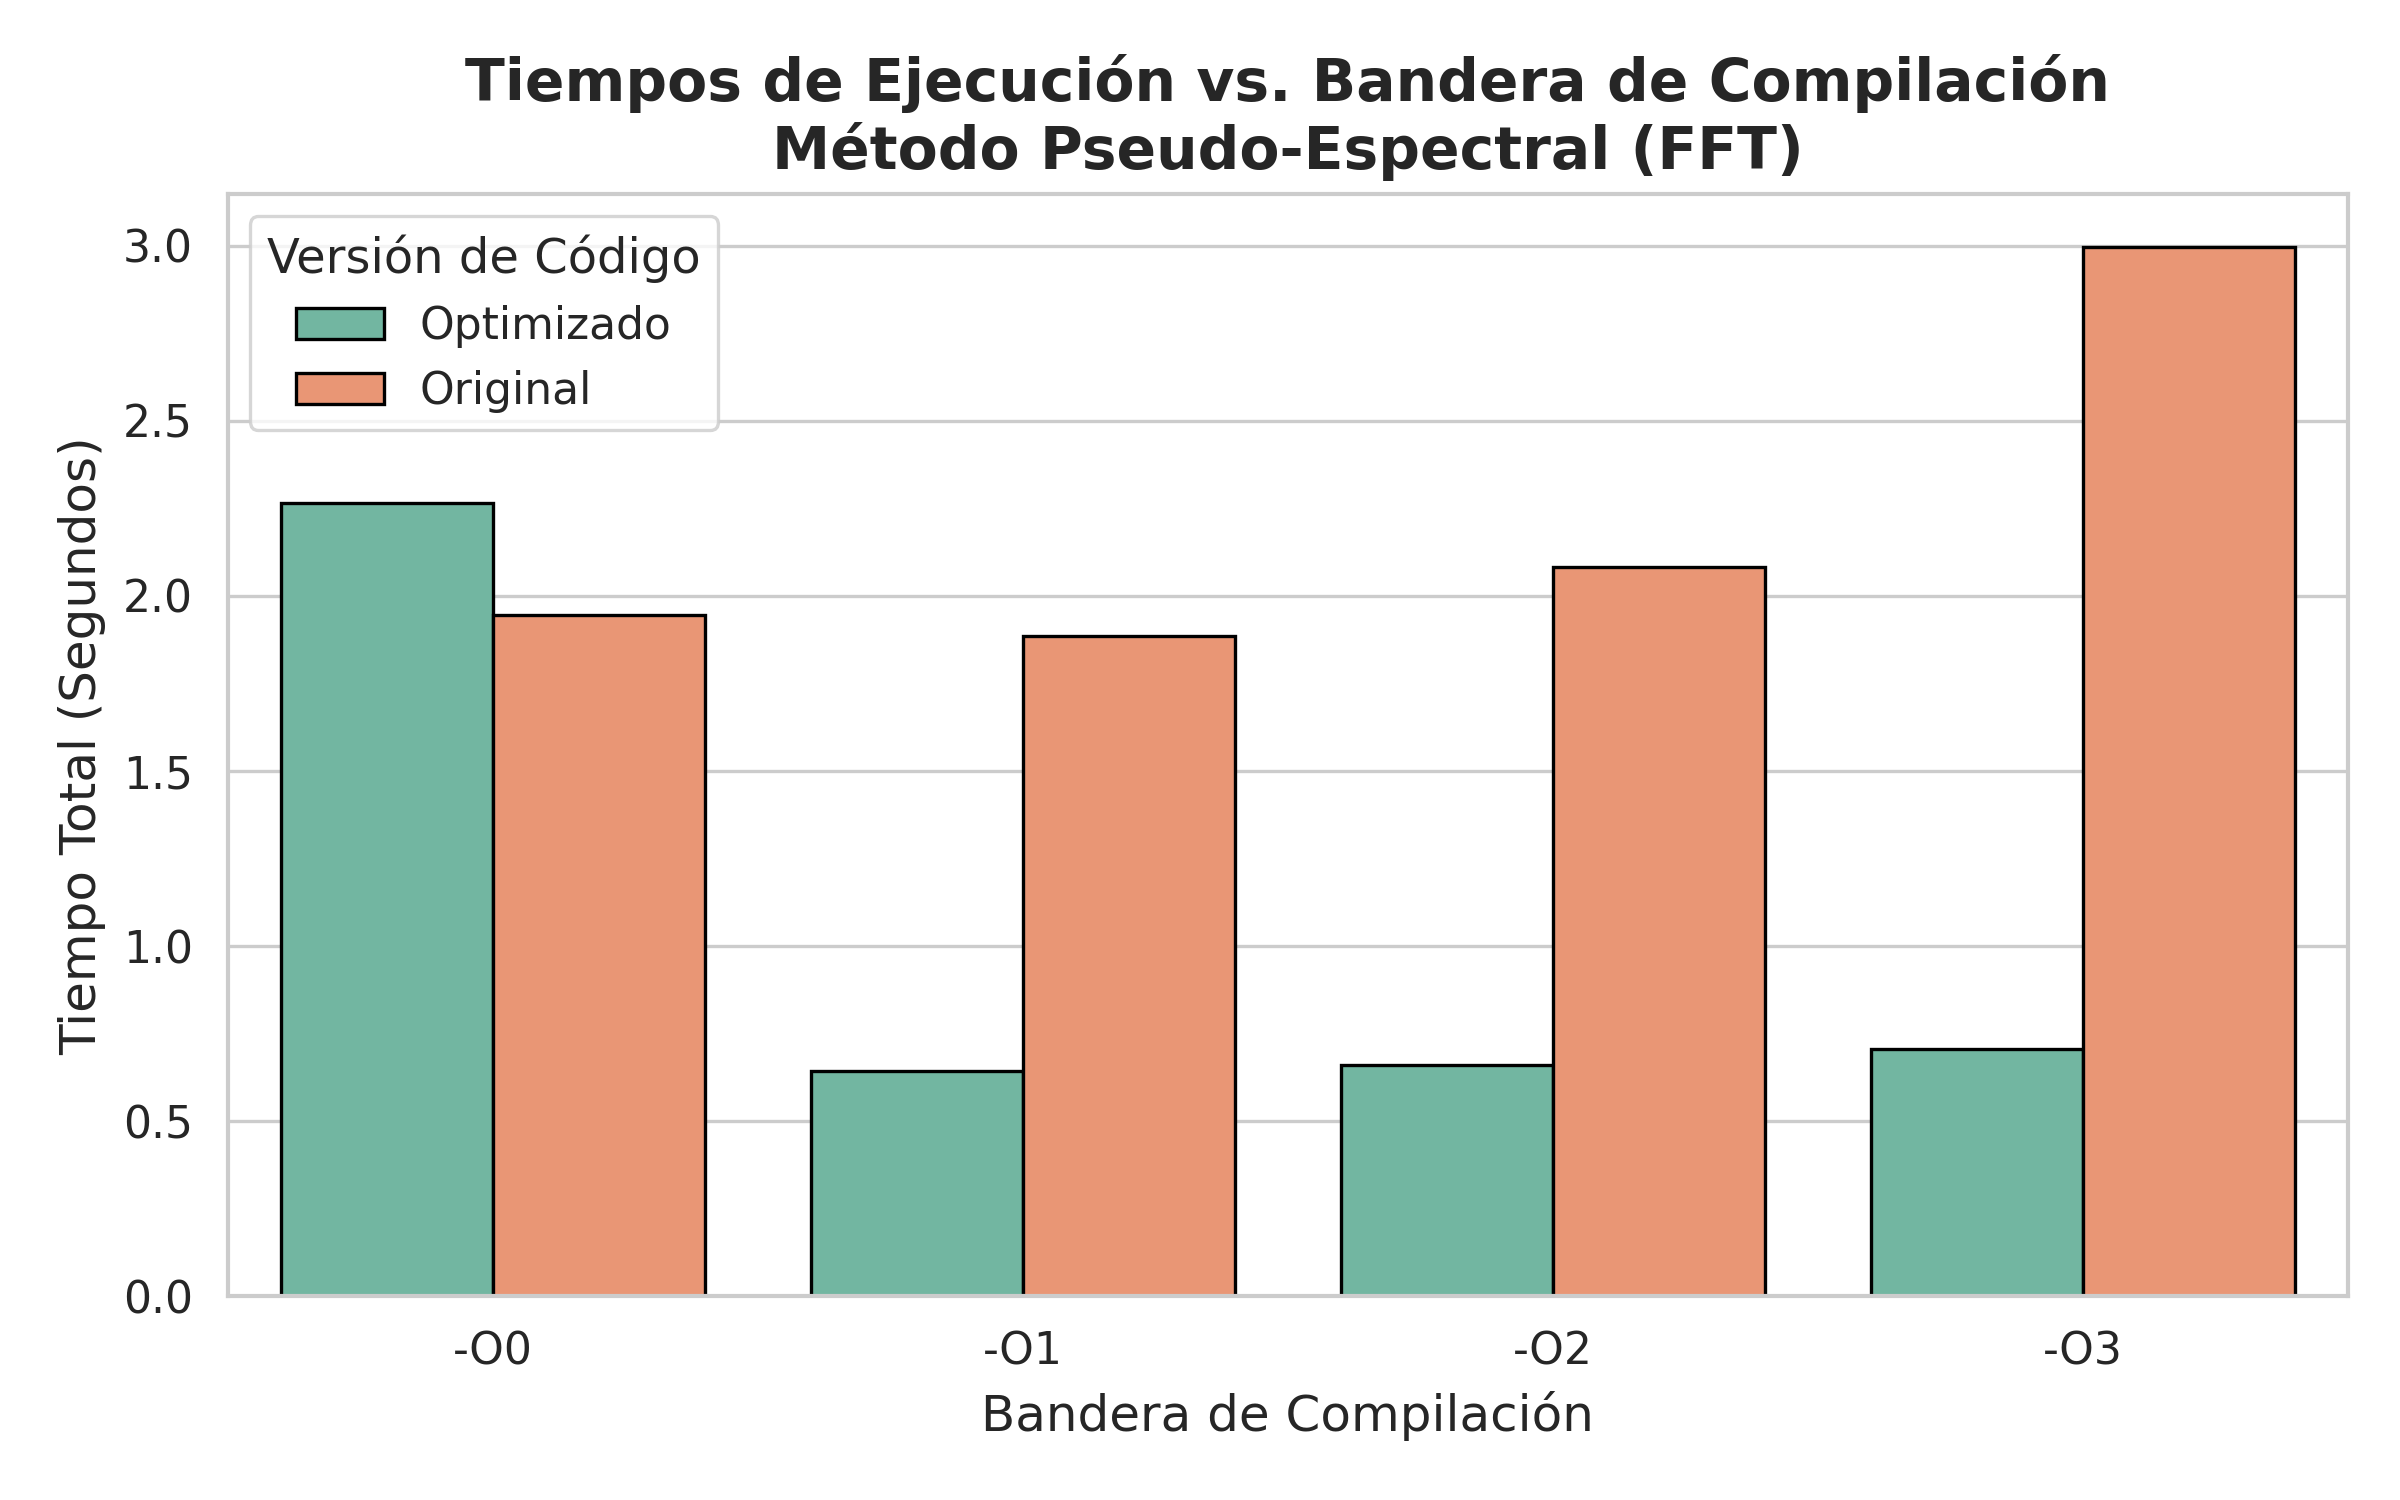
\includegraphics[width=0.48\linewidth]{../../img/barras_optimizacion_code1.png}
        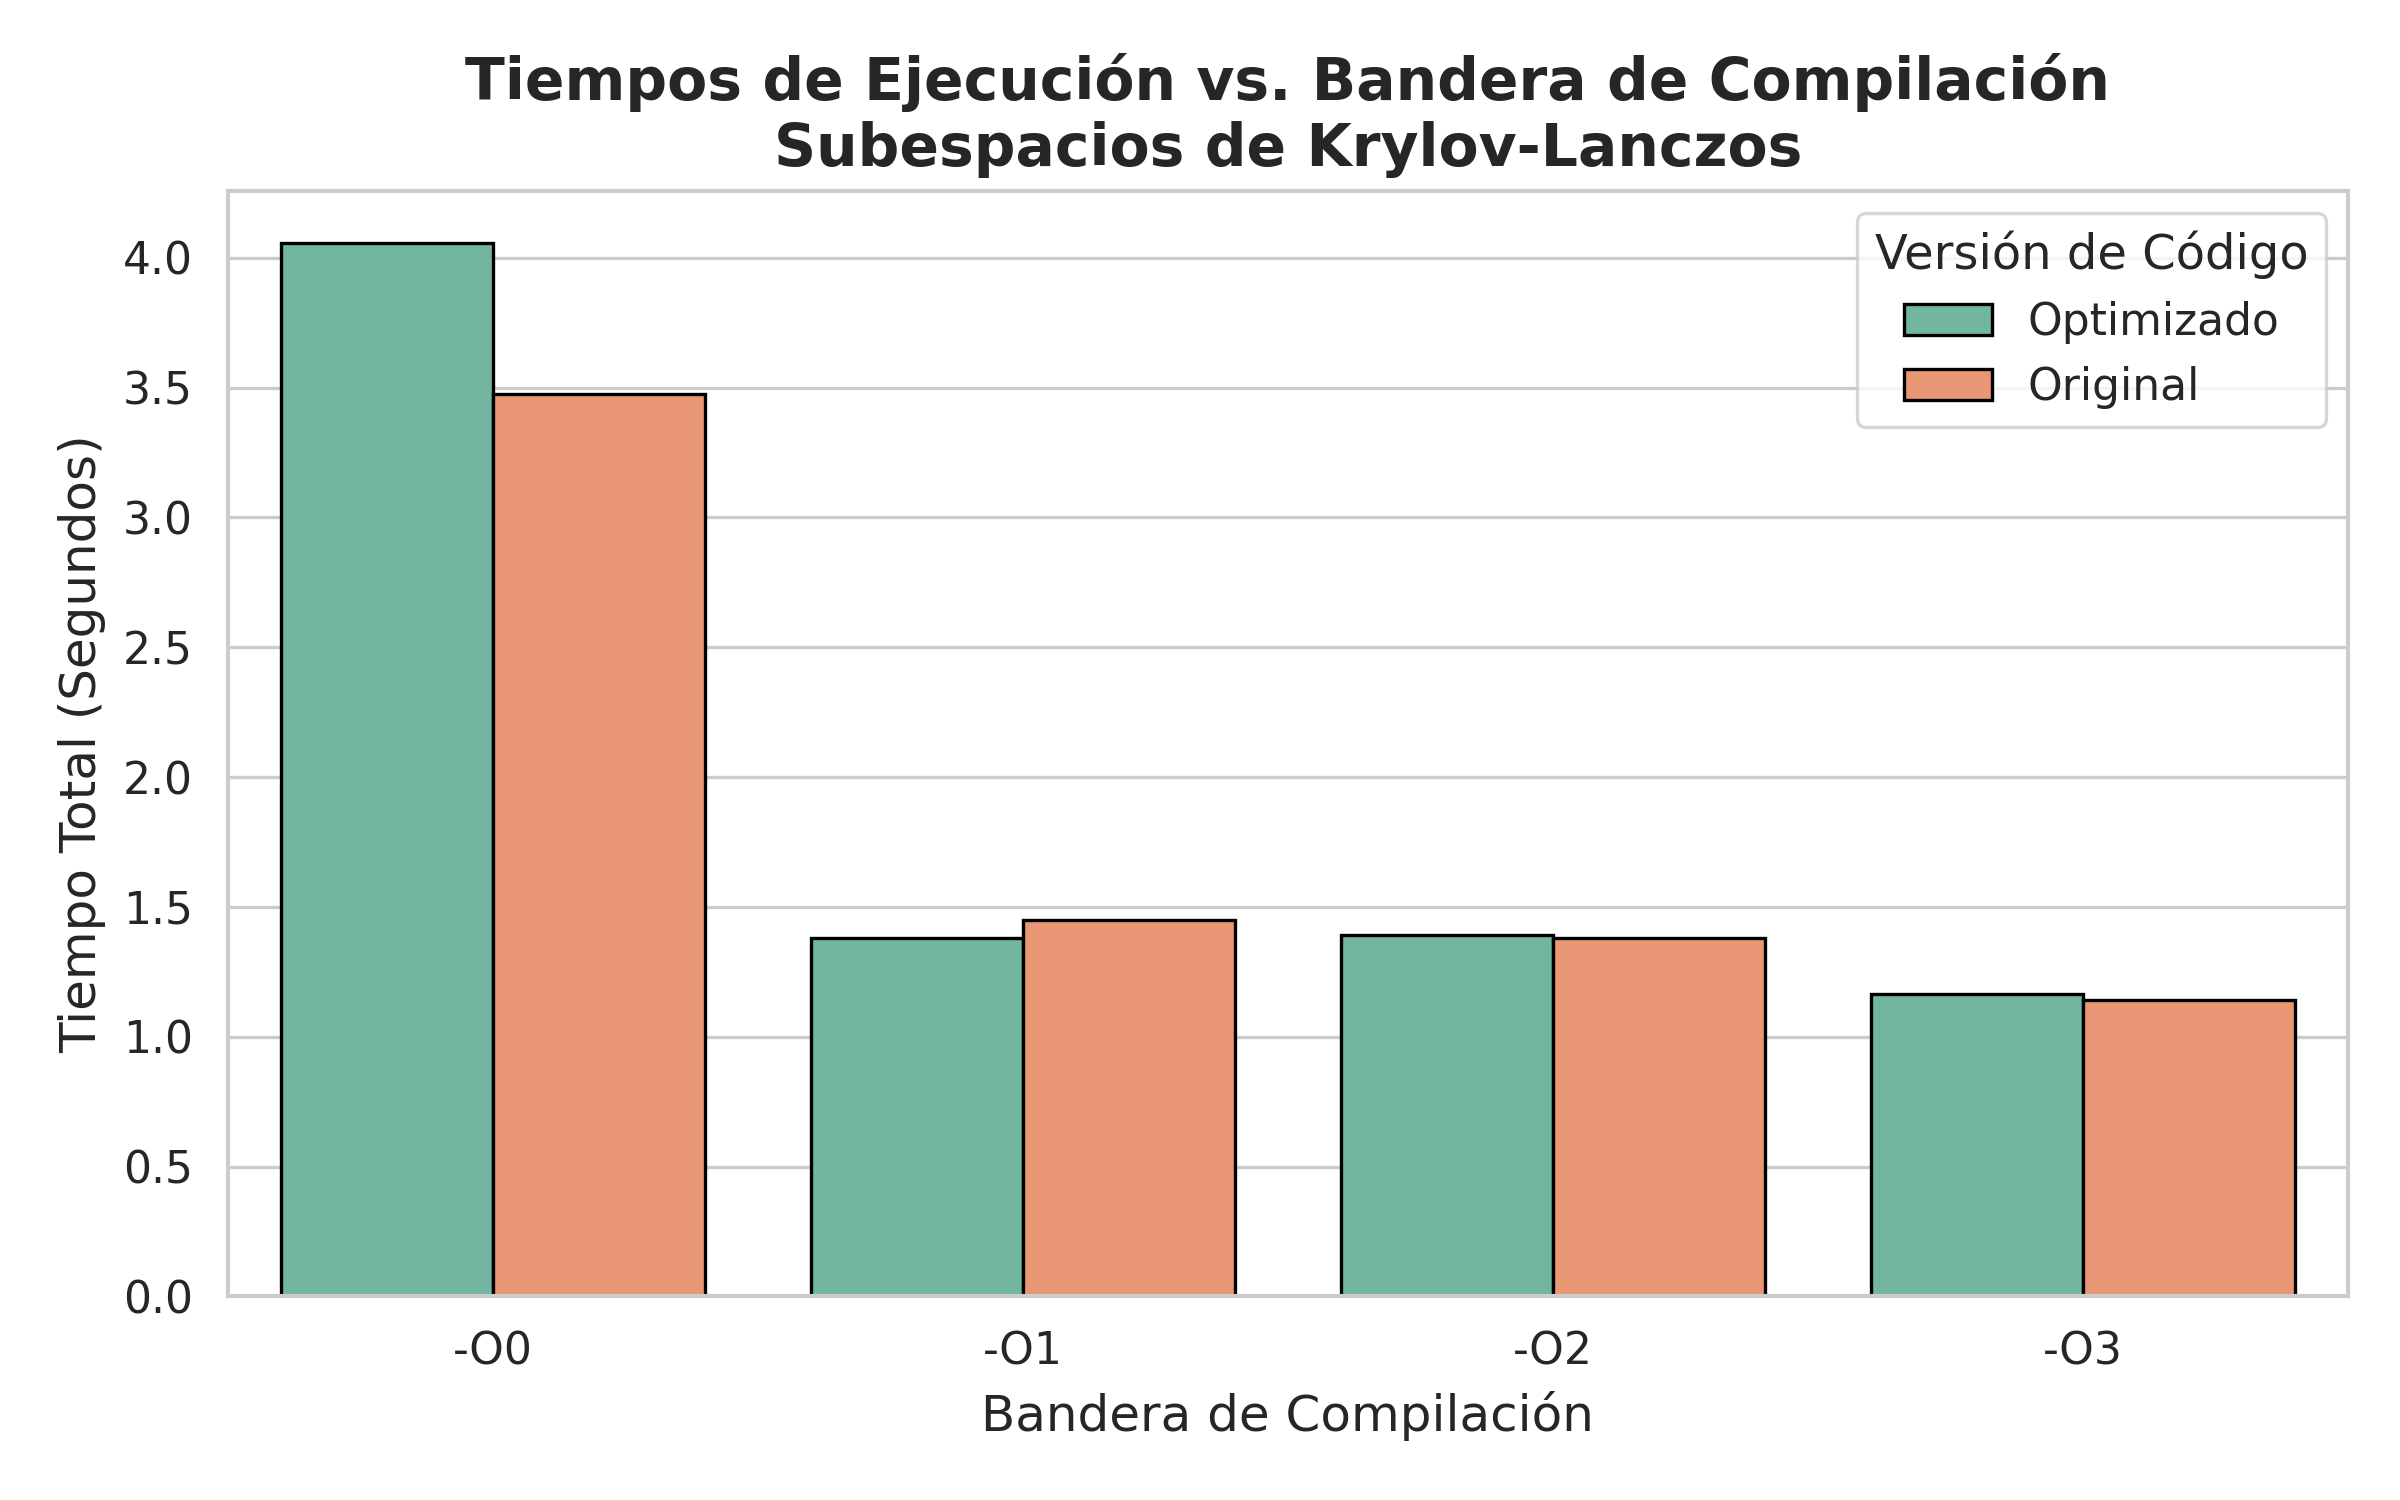
\includegraphics[width=0.48\linewidth]{../../img/barras_optimizacion_code4.png}
        \caption{Impacto de banderas (-O0 a -O3) en métodos no-locales (izq) y locales (der).}
      \end{figure}
    \column{0.43\textwidth}
      \begin{block}{Banderas de Compilación}
        Saltar de \texttt{-O0} a \texttt{-O3} redujo tiempos drásticamente (hasta $67\%$ en Lanczos) por vectorización SIMD y mapeo en registros.
      \end{block}
      \begin{alertblock}{La ilusión del Tiling}
        Aplicar reestructuración espacial (Blocking) fue \textbf{crucial} para arreglar la FFT. Sin embargo, fracasó en Lanczos/Chebyshev. ¿Por qué?\\
        Para $N=2048$, el arreglo completo ($\sim 32$ KB) ya cabía holgadamente en la \textbf{caché L1D} (2 MiB) del procesador AMD Threadripper.
      \end{alertblock}
  \end{columns}
\end{frame}

% ============================================================
\section{Paralelización OpenMP}
% ============================================================

\begin{frame}[fragile]{Paralelización con OpenMP y Prevención de Carreras}
  \begin{columns}[c]
    \column{0.55\textwidth}
\begin{lstlisting}[language={[90]Fortran},caption={Cálculo de norma - Método Krylov-Lanczos}]
dot_prod_real = 0.0_dp
dot_prod_imag = 0.0_dp

!$omp parallel do reduction(+:dot_prod_real, dot_prod_imag) &
!$omp private(i, dot_prod_local) shared(psi, npts) default(none)
do i = 1, npts-1
  dot_prod_local = conjg(psi(i)) * psi(i)
  dot_prod_real = dot_prod_real + real(dot_prod_local, dp)
  dot_prod_imag = dot_prod_imag + aimag(dot_prod_local)
end do

norm_psi = sqrt(dot_prod_real * dx)
\end{lstlisting}
    \column{0.43\textwidth}
      \begin{block}{Rigurosidad en el Alcance}
        Se utilizó explícitamente \texttt{default(none)} para obligar a clasificar cada variable, mitigando accesos concurrentes indebidos.
      \end{block}
      \begin{exampleblock}{Reduction}
        Las variables \texttt{dot\_prod\_real} e \texttt{imag} se declararon en cláusula de \emph{reduction} para asegurar una suma paralela libre de \textit{race conditions}.
      \end{exampleblock}
  \end{columns}
\end{frame}

\begin{frame}{Métricas HPC: Escalabilidad y Ley de Amdahl}
  \begin{columns}[c]
    \column{0.65\textwidth}
      \begin{figure}
        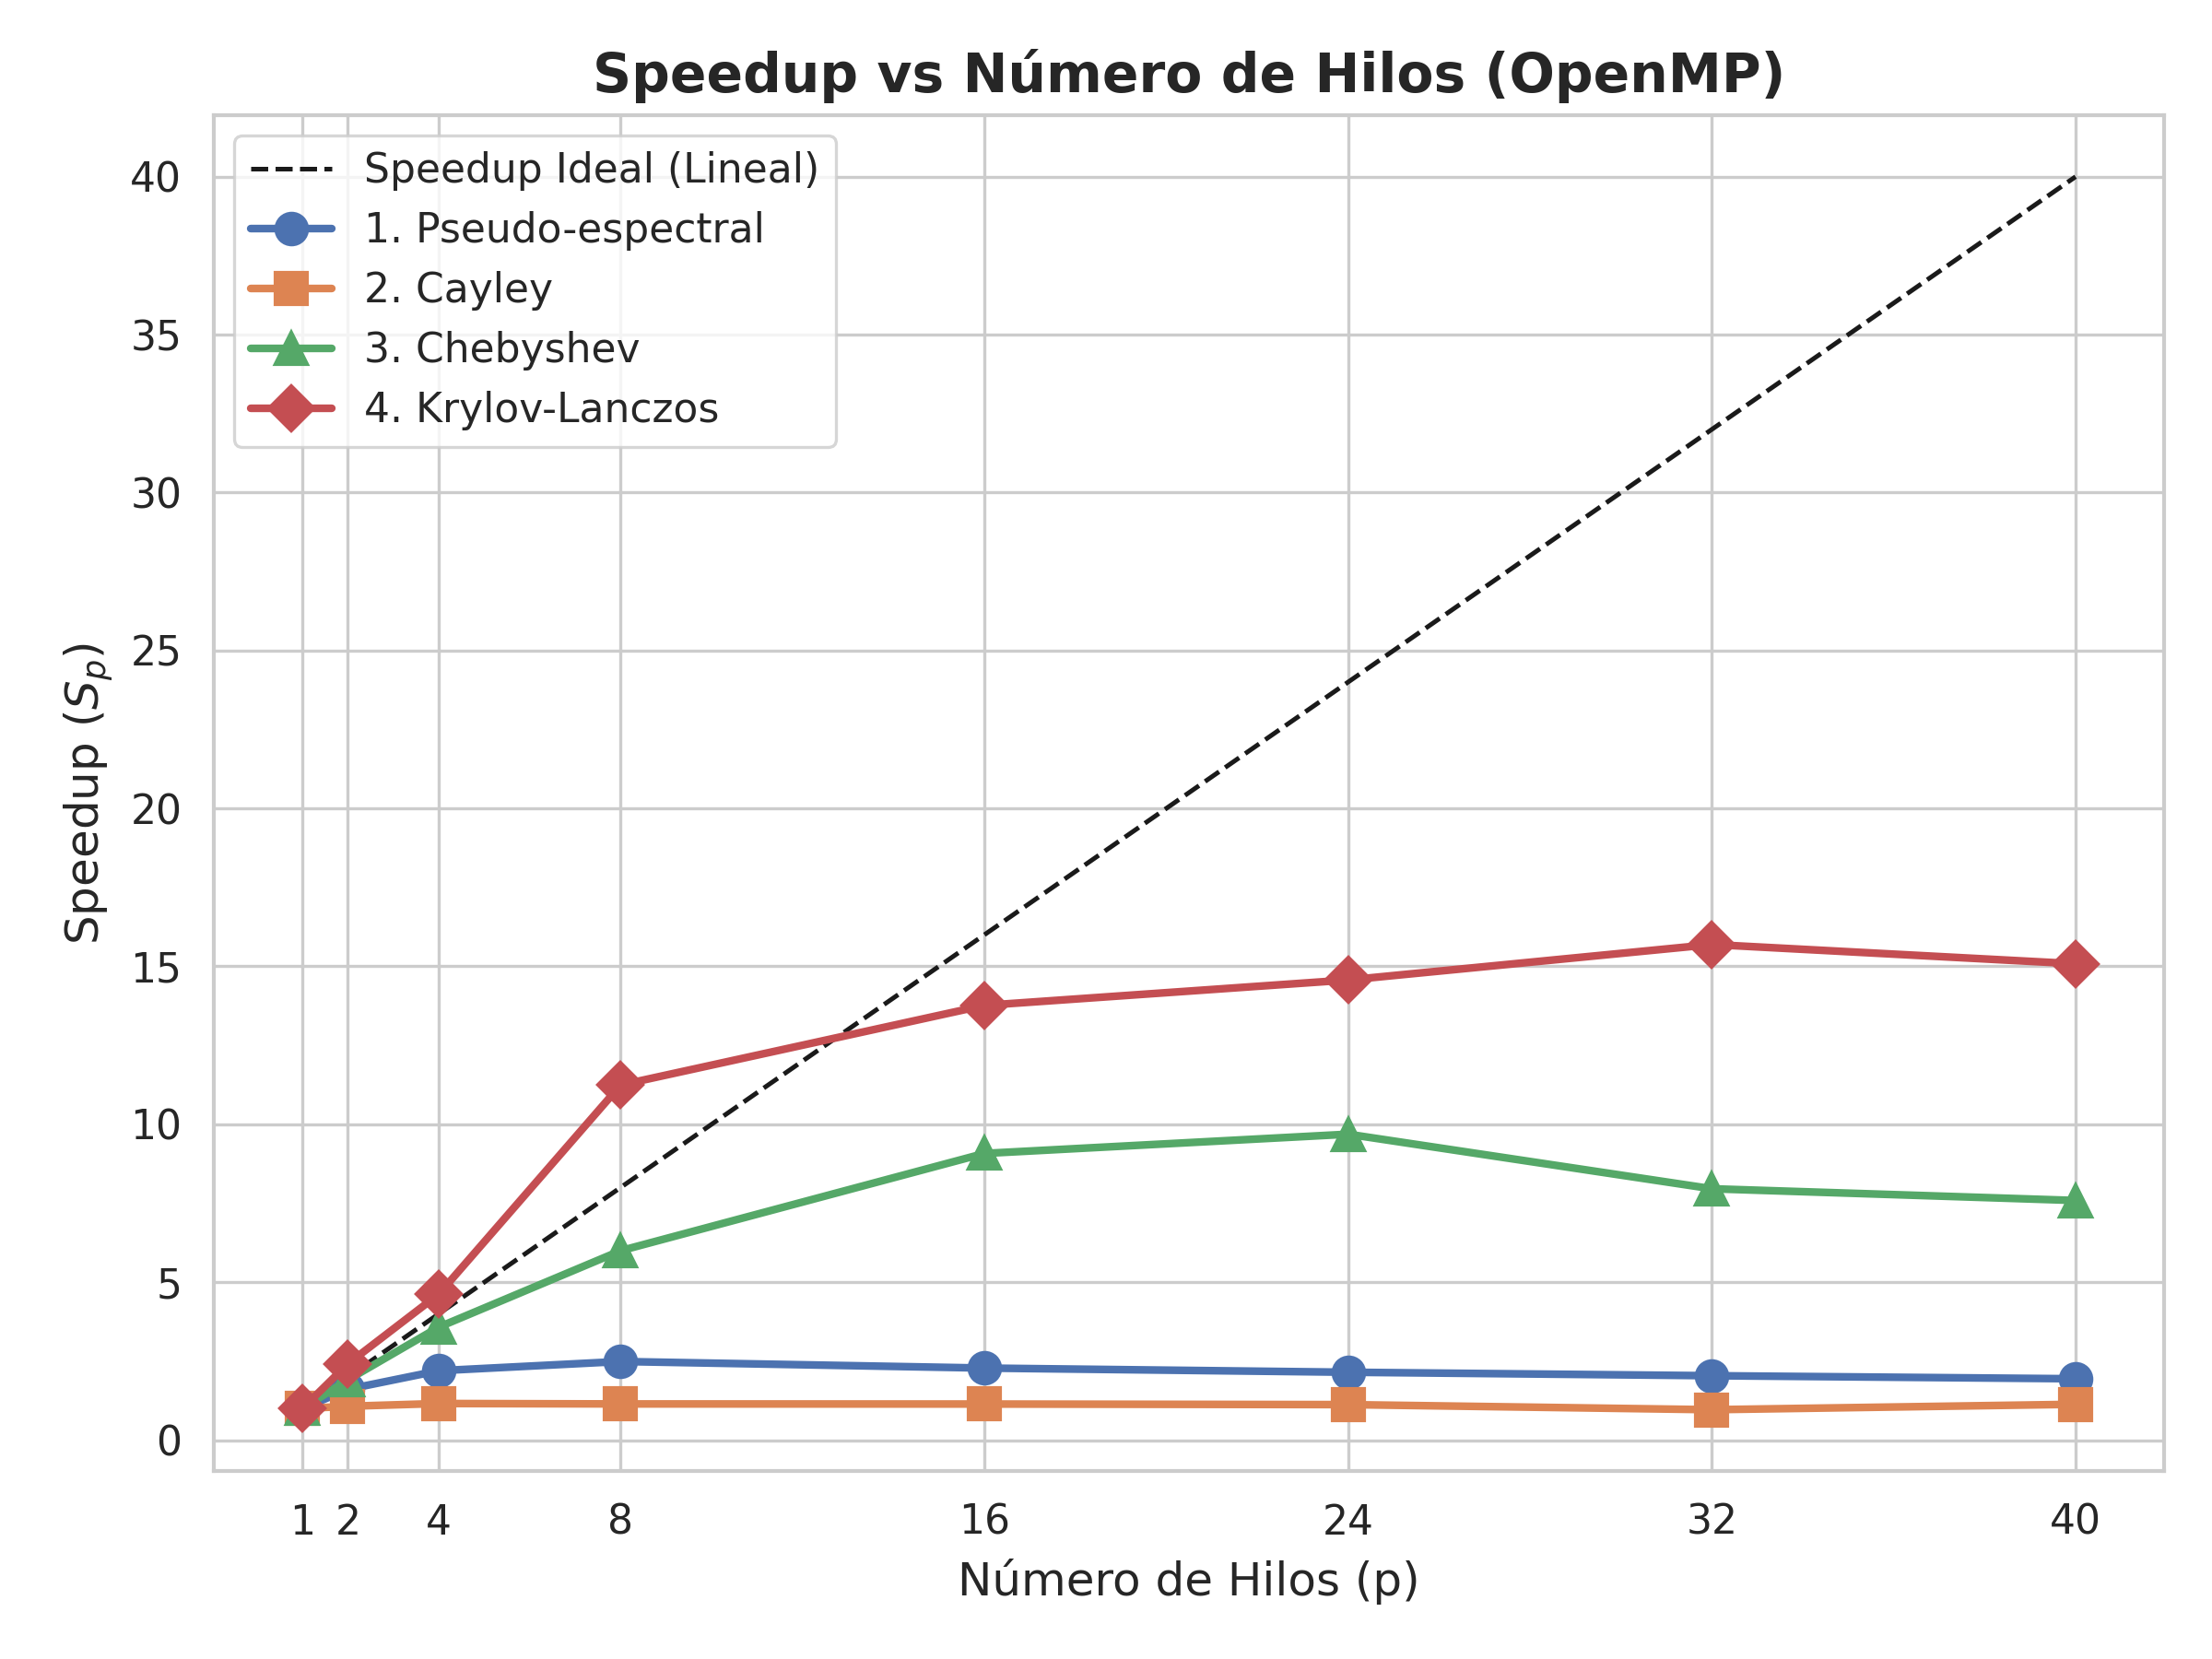
\includegraphics[width=0.49\linewidth]{../../img/openmp_speedup_comparativo.png}
        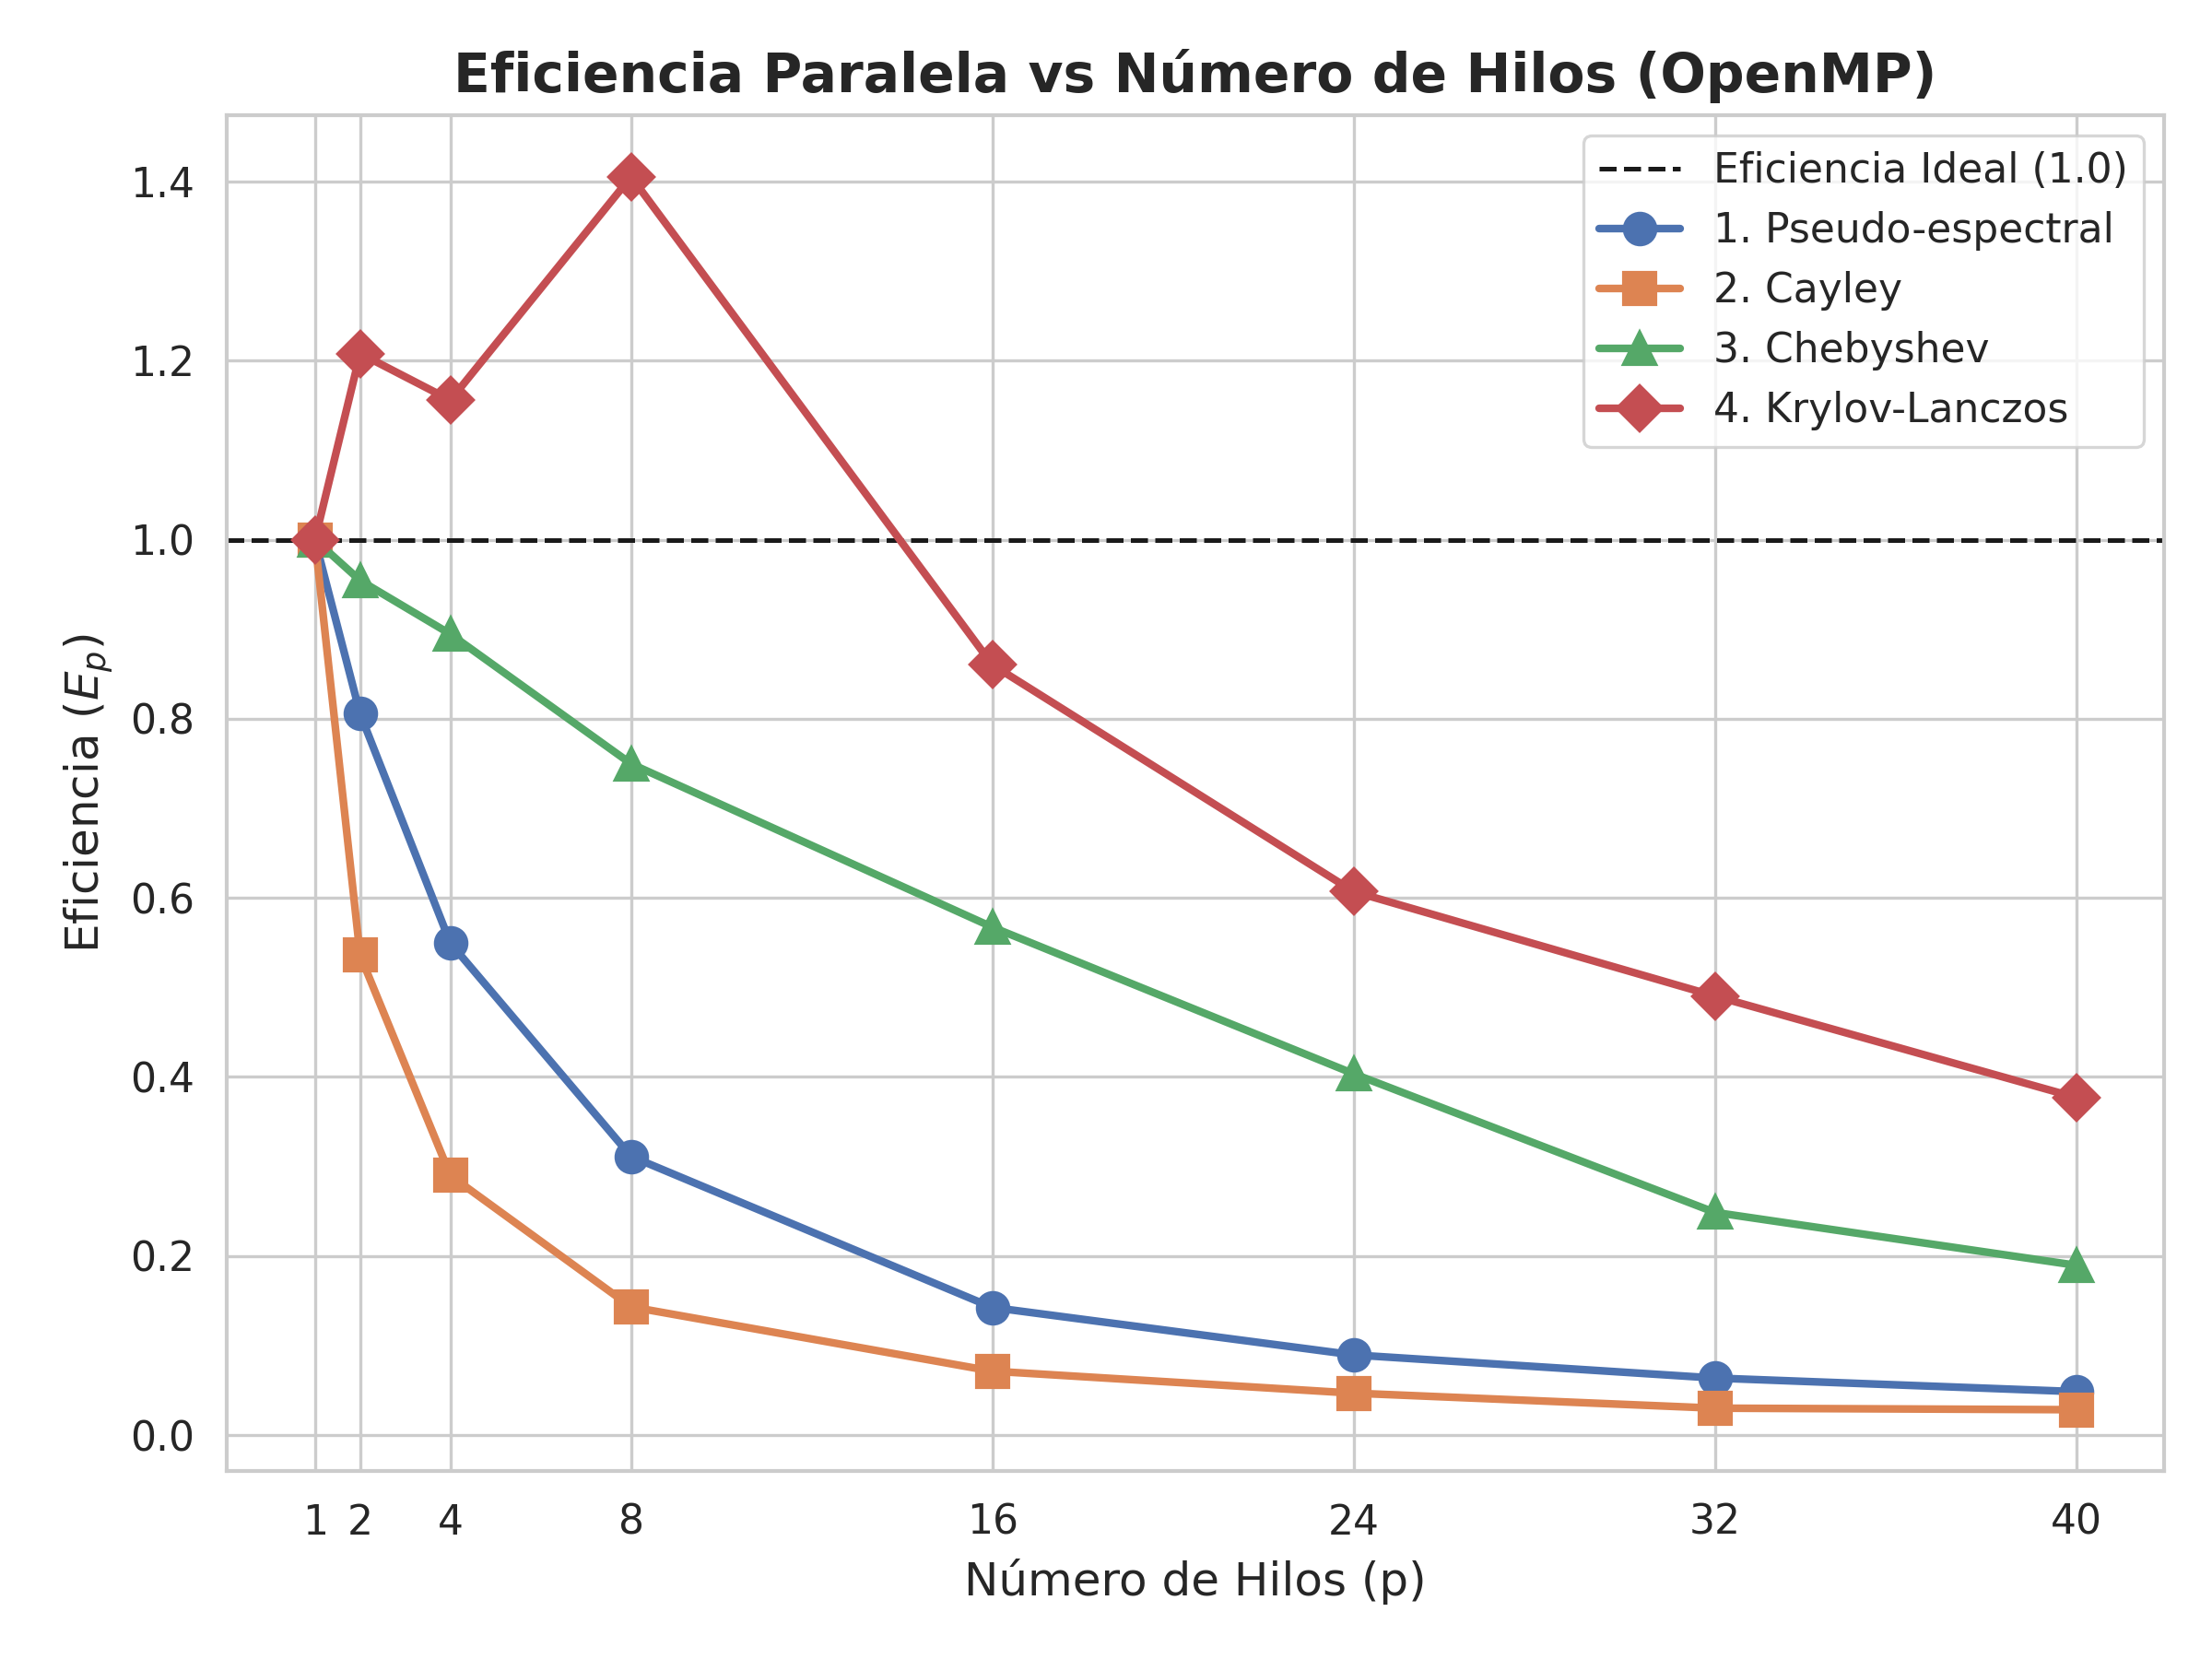
\includegraphics[width=0.49\linewidth]{../../img/openmp_eficiencia_comparativa.png}
      \end{figure}
    \column{0.33\textwidth}
      \begin{block}{Lanczos: Speedup Superlineal}
        A 4 hilos, $S_4 = 4.62$ ($E_p > 1.0$). Al dividir la malla, los subconjuntos (\textit{working set}) caben enteros en la caché ultra rápida.
      \end{block}
      \begin{alertblock}{Fracaso de Cayley}
        Estancado en $1.16\times$. La resolución de sistemas tridiagonales impuso dependencias fatales. Por Ley de Amdahl, su fracción serial arruina la escalabilidad.
      \end{alertblock}
  \end{columns}
\end{frame}

% ============================================================
\section{Validación Física}
% ============================================================

\begin{frame}{Validación Física del Modelo}
  \begin{columns}[c]
    \column{0.55\textwidth}
      \begin{figure}
        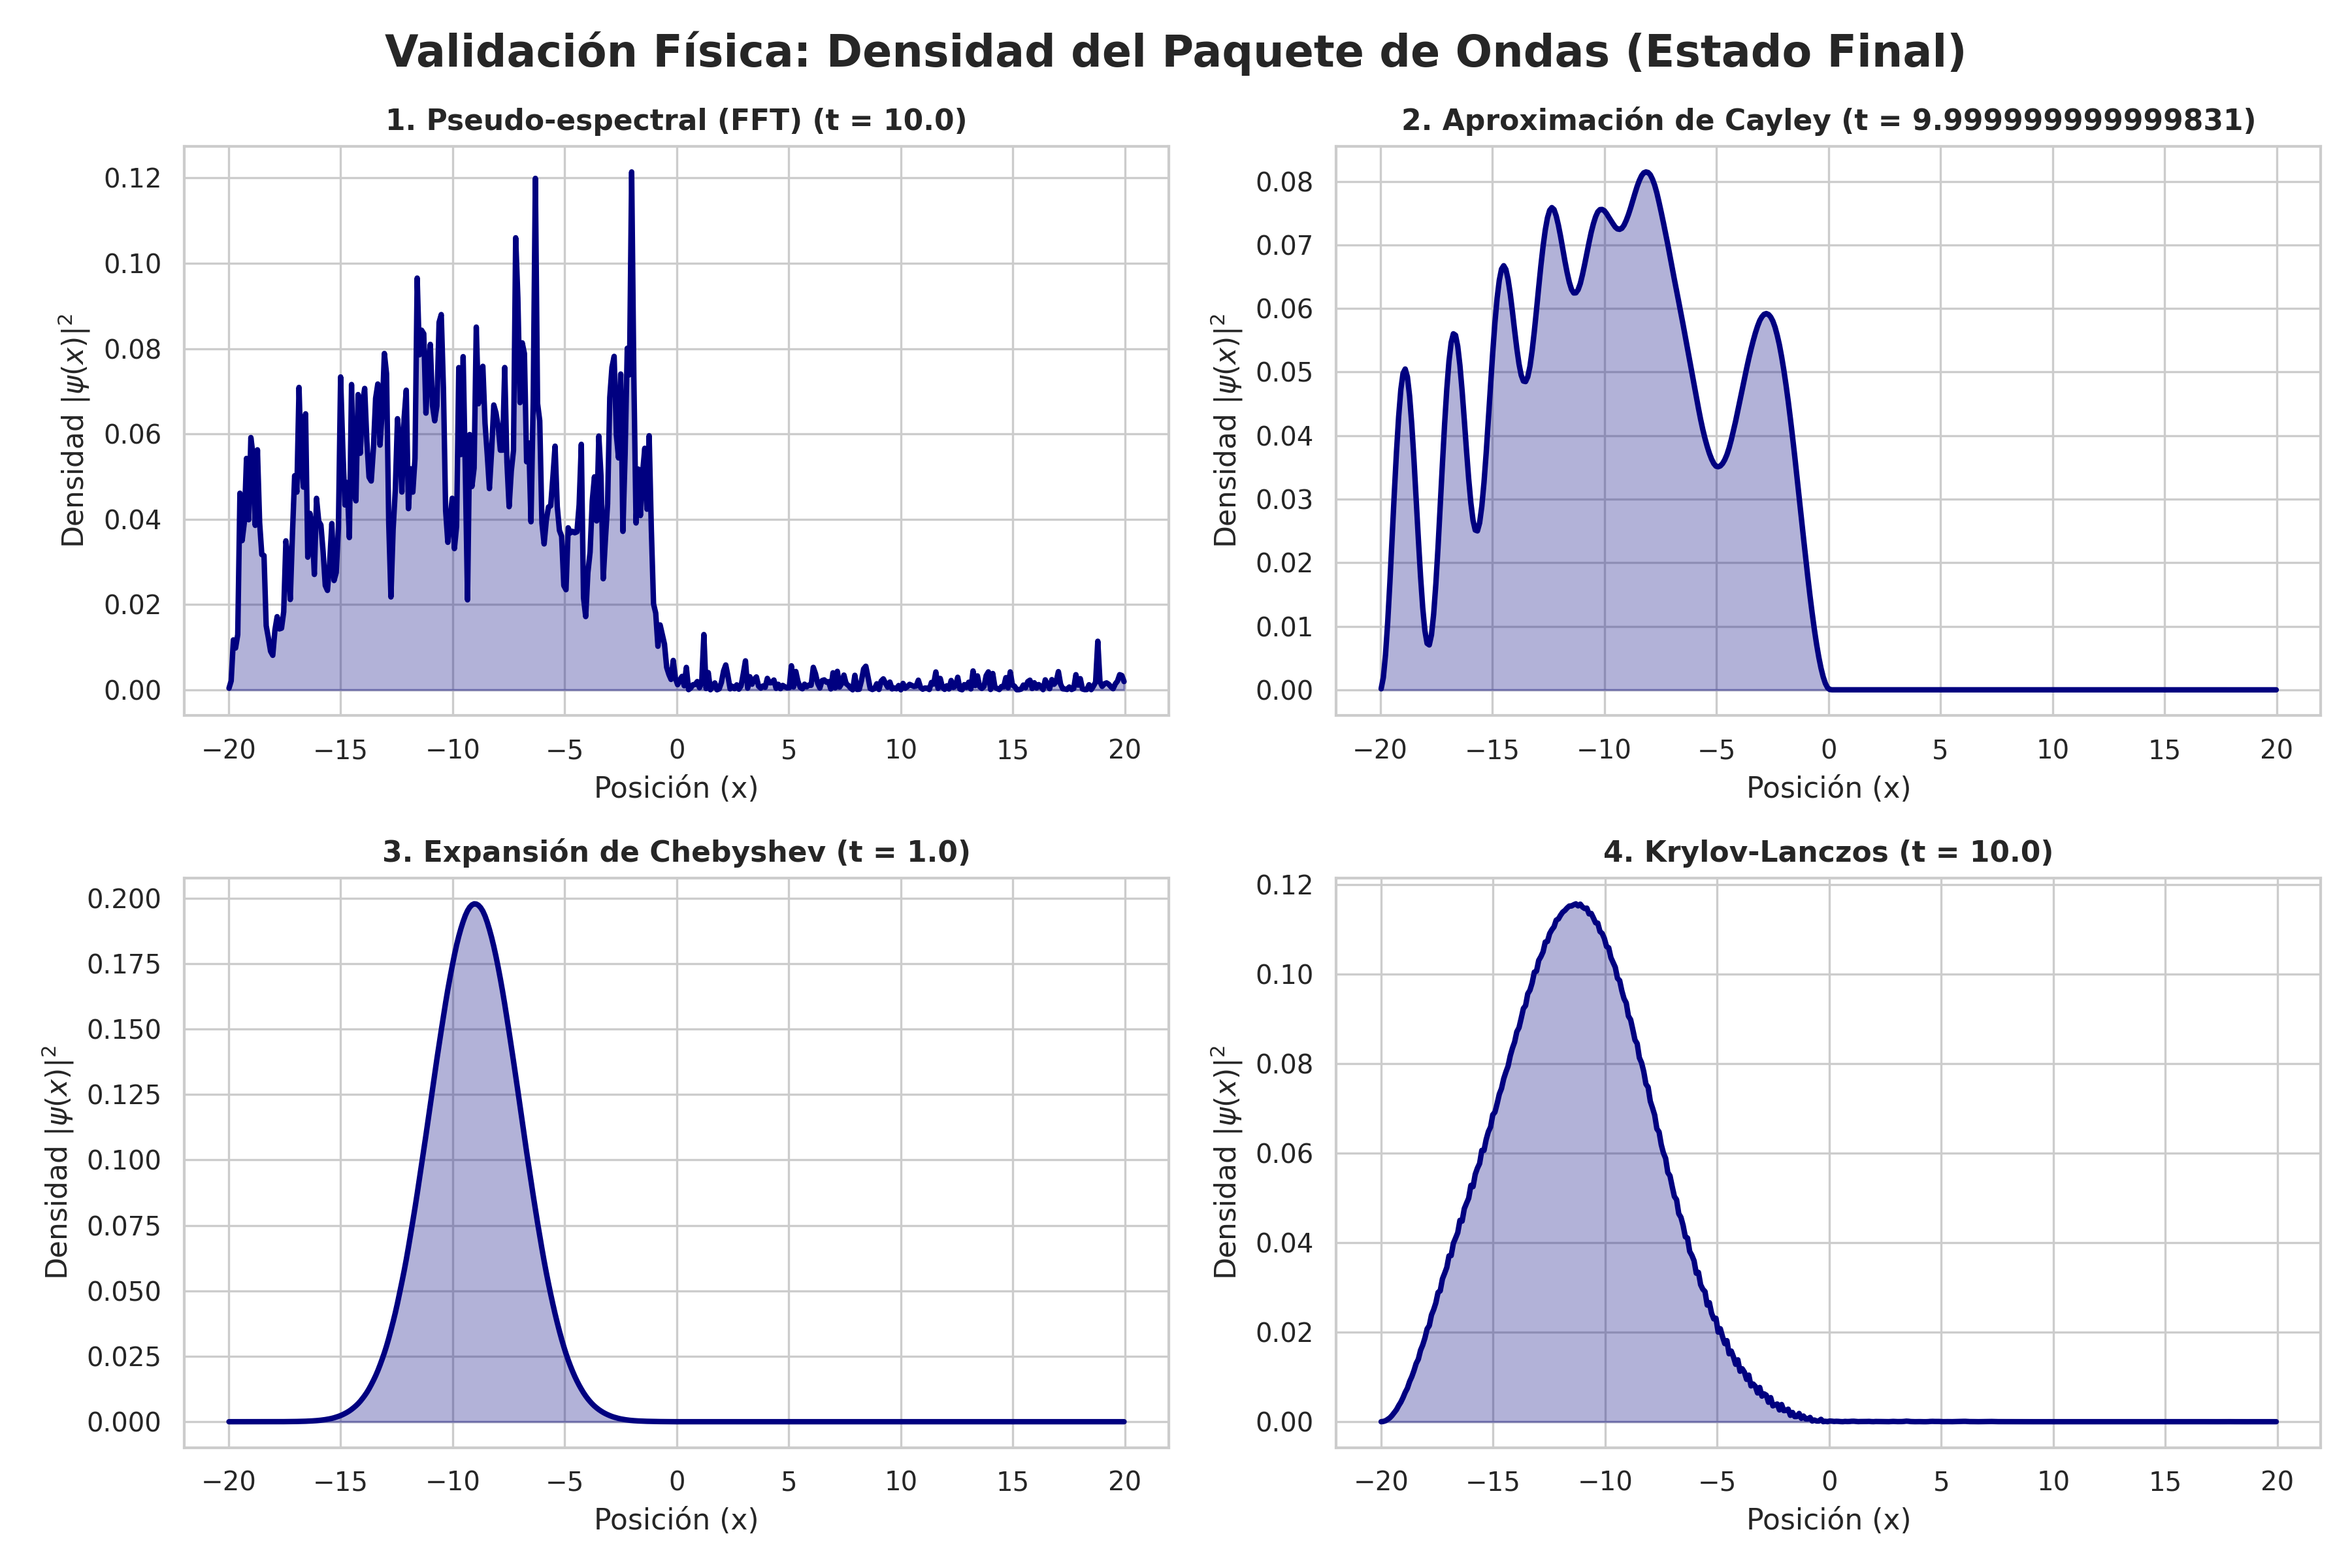
\includegraphics[width=1.0\linewidth]{../../img/fisica_densidad_final.png}
        \caption{Densidad de probabilidad en etapa final.}
      \end{figure}
    \column{0.43\textwidth}
      \begin{block}{La trampa de la probabilidad}
        Todos conservan la norma en $1.0$, pero ¿hacen la misma física?
      \end{block}
      \begin{alertblock}{Distorsiones Numéricas}
        \begin{itemize}
            \item \textbf{FFT:} \textit{Aliasing} masivo al tocar los bordes por sus condiciones periódicas intrínsecas.
            \item \textbf{Cayley:} Sufre \textit{dispersión numérica}. Diferentes velocidades de fase desgarran el paquete.
        \end{itemize}
      \end{alertblock}
      \begin{exampleblock}{La victoria de Lanczos}
        Expansión gaussiana natural y limpia, sin ruido numérico.
      \end{exampleblock}
  \end{columns}
\end{frame}

% ============================================================
\section{Conclusiones}
% ============================================================

\begin{frame}{Análisis Comparativo Integral}
  \begin{columns}[t]
    \column{0.48\textwidth}
      \begin{block}{1. Algoritmo vs Arquitectura}
        Métodos como Cayley, aunque unitarios en papel, son inviables en HPC. Las matemáticas de resolución tridiagonal limitan la paralelización masiva.
      \end{block}
      \begin{block}{2. Conciencia de Caché}
        Reestructurar bucles (Tiling) arregla accesos a memoria erráticos (FFT), pero añade latencia perjudicial a operadores locales que ya caben en la caché L1/L2.
      \end{block}
    \column{0.48\textwidth}
      \begin{exampleblock}{3. El veredicto: Krylov-Lanczos}
        La eficiencia computacional no debe sacrificar la integridad física.\\
        \vspace{0.2cm}
        \textbf{Krylov-Lanczos} emergió como la solución definitiva:
        \begin{itemize}
            \item Escalabilidad paralela superlineal.
            \item Localidad de datos perfecta en memoria.
            \item Evolución física impecable sin dispersión ni aliasing.
        \end{itemize}
      \end{exampleblock}
  \end{columns}
  
  \vspace{0.3cm}
  \begin{center}
    \begin{tikzpicture}
      \node[fill=UDprimary,text=white,rounded corners=4pt,
            inner xsep=12pt,inner ysep=6pt,font=\bfseries\small] {
        Conclusión: Escribir código rápido requiere respetar incondicionalmente la dinámica del sistema.
      };
    \end{tikzpicture}
  \end{center}
\end{frame}

% ─── DIAPOSITIVA DE CIERRE ────────────────────────────────────
{
\setbeamertemplate{headline}{}
\setbeamertemplate{footline}{}
\begin{frame}[plain]
  \begin{tikzpicture}[remember picture,overlay]
    \fill[UDprimary] (current page.south west) rectangle (current page.north east);
    \fill[UDdark,opacity=0.4]
      (current page.south west) rectangle (current page.north east);
    \fill[UDsecond,opacity=0.85]
      ([xshift=-0.08\paperwidth]current page.north east) rectangle
      (current page.south east);
    \draw[UDlight,line width=1.5pt]
      ([yshift=-0.45\paperheight]current page.north west) --
      ([yshift=-0.45\paperheight,xshift=-0.08\paperwidth]current page.north east);
  \end{tikzpicture}

  \begin{center}
    \vspace{0.8cm}
    {\color{white}\Huge\bfseries ¡Gracias!}\\[10pt]
    \color{white}\rule{0.5\textwidth}{0.4pt}\\[10pt]
    {\color{UDlight}\large Camilo Huertas \quad · \quad Sebastián Rodriguez}\\[6pt]
    {\color{UDlight}\small Proyecto Curricular de Física}\\
    {\color{UDlight}\small Universidad Distrital Francisco José de Caldas}\\[6pt]
    {\color{UDlight}\footnotesize Docente: Carlos Andrés Gómez Vasco \quad|\quad Computación de Alto Desempeño}
  \end{center}
\end{frame}
}

\end{document}
